%!TEX TS-program = ../make.zsh

\newcommand\done{\checkmark\xspace}
\newcommand\inprogress{$\Rightarrow$\xspace}
\newcommand\tobedone{$\square$\xspace}

\section{Overview}
\subsection{Goal and Context}
\begin{frame}[fragile]{Overview: Goal and Context}
  \begin{columns}
    \begin{column}{0.65\textwidth}
      \begin{description}
        \item[Origin] \her{Master thesis} (2018-09) implementing direct photon propagation through hole ice in clsim in order to study hole-ice effects and improve understanding of low-energy systematics. \small \url{https://github.com/fiedl/hole-ice-study} \normalsize

        \item[Goal] \her{Bring} the new simulation \her{into} the icecube-simulation \her{framework} such that other icecubers can use it.

        \item[Context] \her{Service work} for the icecube collaboration in the beginning of my time as PhD student with icecube at ECAP/Erlangen.

        \item[Time frame] about 6 months
      \end{description}

      \source{\underline{Top}: Rongen: The 2018 Sweden Camera run — light at the end of the ice, 2018. \underline{Bottom}: \url{https://github.com/fiedl/hole-ice-study/issues/107}}
    \end{column}
    \begin{column}{0.35\textwidth}
      \image{camera2018-01}

      % https://github.com/fiedl/hole-ice-study/issues/107
      \image{flasher-steamshovel-single-received-photon}
    \end{column}
  \end{columns}
\end{frame}

\subsection{Work to be done}
\begin{frame}{Overview: Work to be done}

  %\begin{itemize}
  %
  %
  %  \item[\done] Compile current icecube-simulation release V06-01-01 with Python 3 locally
  %  \item[\done] Make hole-ice code work with current icecube-simulation release V06-01-01
  %  \item[\inprogress] Provide example scripts for Python 3 (rather than Ruby)
  %  \item[\inprogress] Synchronize svn and git repositories of clsim
  %  \item[\tobedone] Re-implement ice tilt and ice anisotropy
  %  \item[\tobedone] Implement direct-detection switch
  %  \item[\tobedone] Merge hole-ice code into clsim trunk
  %\end{itemize}

  \setbeamertemplate{subsection in toc}{\hspace*{1em} \inserttocsubsection \vspace{2ex} \par}
  \tableofcontents[sectionstyle=hide,subsectionstyle=show,sections=2-]

  \bigskip \bigskip \small
  \done = done \ \ \ \inprogress = work in progress \ \ \ \tobedone\ = still to do
\end{frame}

\section{State of the individual steps}
\subsection{\done Compile IceSim V06-01-01 with Python 3}
\begin{frame}{\done Compile IceSim V06-01-01 with Python 3}
  \begin{itemize}
    \item In Stockholm (2018-09), the icecube software group requested the hole-ice example scripts to be provided in Python 3 (rather than Python 2 or Ruby) in order to push the migration to Python 3 forward.
    \item The current icecube documentation on how to install the framework on macOS still assumes Python 2: \url{http://software.icecube.wisc.edu/documentation/projects/cmake/supported_platforms/osx.html}
    \item First attempt to compile locally on macOS Sierra with Python 3 has failed.
  \end{itemize}
\end{frame}

\begin{frame}[fragile]{\done Compile IceSim V06-01-01 with Python 3}
  \begin{columns}
    \begin{column}{0.5\textwidth}
      \begin{itemize}
        \item<1->[\done] Using Vagrant, a virtual-machine wrapper, I've documented a clean, reproducible way to install icecube-simulation V06-01-01 on macOS Sierra, which I use locally.
        \item<2->[\done] Found a couple of issues and provided patches.
        \item<3->[\tobedone] Still need to talk to the software group. Maybe they want to link or import the install  documentation.
        \item<4->[\tobedone] I would love to run this on Travis-CI. Exposing the build logs (no credentials) to the public would be no problem according to the software group. Unfortunately, the build time exceeds travis' hard limit of 50 minutes.\\
          \tiny \url{https://travis-ci.org/fiedl/hole-ice-install} \\
          \url{https://icecube-spno.slack.com/archives/C02KQL9KN/p1552577601148400}
        \item<5-> \color{blue}{Does anyone know about icecube's build bots? Where are the build scripts? Why didn't they indicate that V06-01-01 does not compile on macOS Sierra?}
      \end{itemize}
    \end{column}
    \begin{column}{0.5\textwidth}
      \begin{onlyenv}<1-3>
        \begin{bash}
          # Clone this repository
          git clone git@github.com:fiedl/hole-ice-install.git

          # .secrets.sh
          export SVN="our svn url"
          export SVN_ICECUBE_USERNAME="our svn username"
          export SVN_ICECUBE_PASSWORD="our svn password"

          # Install Vagrant
          brew cask instal vagrant

          # Start the virtual machine and run the install instructions
          vagrant up
        \end{bash}

        \bigskip \her{Documented at: \url{https://github.com/fiedl/hole-ice-install}}
      \end{onlyenv}
      \begin{onlyenv}<4>
        \begin{bash}
          [ 87%] Building CXX object polyplopia/private/pybindings/CMakeFiles/polyplopia-pybindings.dir/PolyplopiaUtils.cxx.o
          [ 87%] Building CXX object MuonGun/CMakeFiles/MuonGun-pybindings.dir/private/pybindings/EnergyDistribution.cxx.o
          [ 87%] Building CXX object clsim/CMakeFiles/clsim.dir/private/clsim/function/I3CLSimFunctionScatLenIceCube.cxx.o
          [ 87%] Building CXX object steamshovel/CMakeFiles/shovelart-pybindings.dir/private/scripting/pytypename.cpp.o
          [ 87%] Building CXX object MuonGun/CMakeFiles/MuonGun-pybindings.dir/private/pybindings/WeightCalculator.cxx.o
          The job exceeded the maximum time limit for jobs, and has been terminated.
        \end{bash}

        \small \url{https://travis-ci.org/fiedl/hole-ice-install} \normalsize
      \end{onlyenv}

      \only<5>{
        \url{http://builds.icecube.wisc.edu}
      }

    \end{column}
  \end{columns}
\end{frame}

\subsection{\inprogress Port hole-ice code to clsim of icecube-simulation V06-01-01}
\begin{frame}{\inprogress Port hole-ice code to clsim of icecube-simulation V06-01-01}
  \begin{itemize}
    \item The original study was based on the icecube-simulation framework V05-00-07 from 2016.
    \item From the V05-00-07 (2016) to V06-01-01 (2019), there are 93 commits in clsim. A lot has changed.
    \item There are two separate repositories for original clsim, in addition to the hole-ice fork, which need to be kept in sync. For my work, I have forked Claudio's repository on github. But now, Claudio's github repository is behind the current work in the SVN repository. \\
      \url{http://code.icecube.wisc.edu/svn/projects/clsim} \\
      \url{https://github.com/claudiok/clsim} \\
      \url{https://github.com/fiedl/clsim}
    \item[\done] Find common interface to sync the repositories: \texttt{git-svn}
    \item[\done] Coordinate with the clsim maintainer, Claudio Kopper: The repositories need to be synced before the code can be ported to avoid conflicts later.
    \item[\inprogress] Rebase the hole-ice changes onto the V06-01-01 release
    \item[\tobedone] Make sure everything is still running
    \item[\tobedone] Make sure there are no conflicts with other attempt on cable shadows
  \end{itemize}
\end{frame}

\subsection{\tobedone Provide example scripts for Python 3}
\begin{frame}[fragile]{\tobedone Provide example scripts for Python 3}
  \begin{columns}
    \begin{column}{0.5\textwidth}
      \begin{itemize}
        \item The example scripts of the original hole-ice study are written in Ruby: \url{https://github.com/fiedl/hole-ice-study}
        \item Icecubers prefer Python instead.
        \item[\inprogress] Together with the calibration group and the POCAM group in Munich, I'm working on a series of hole-ice simulations to study proposed geometries for the icecube upgrade.
        \item[\tobedone] The scripts will be migrated to Python 3, documented, and provided as example scripts for the collaboration.
      \end{itemize}
    \end{column}
    \begin{column}{0.5\textwidth}
      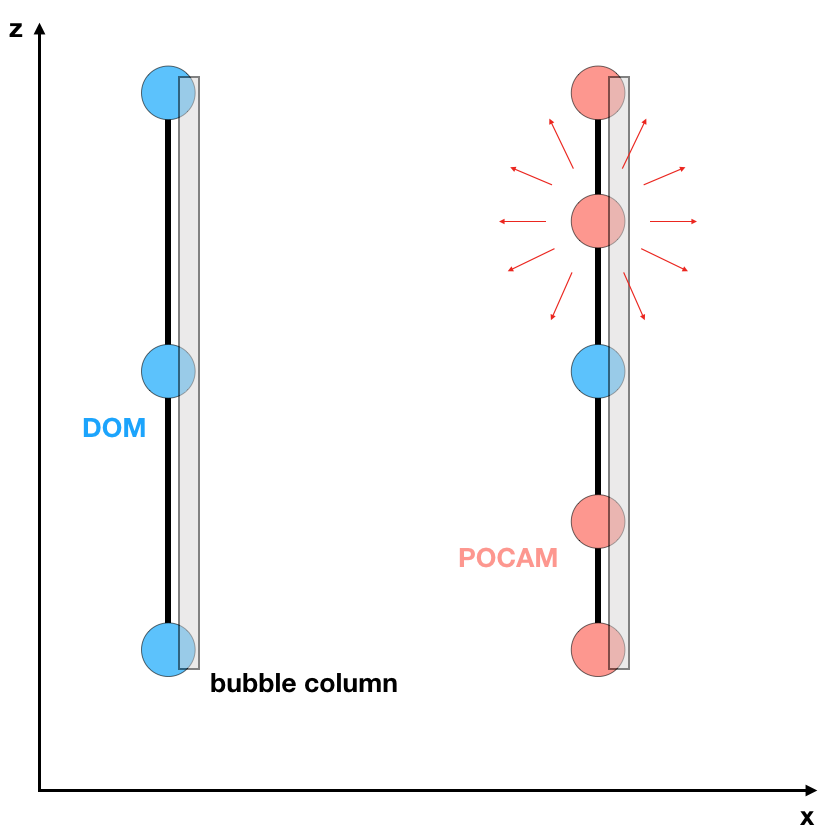
\includegraphics[width=0.8\textwidth]{img/pocamscenario-right}
    \end{column}
  \end{columns}

  \bigskip \her{Example scripts will be at: \url{https://github.com/fiedl/hole-ice-scripts}} \bigskip

  \source{\url{https://github.com/fiedl/hole-ice-talk/releases/tag/v1.5}}
\end{frame}

\begin{frame}{\tobedone Python 3 and IceCube Simulation}
  \begin{itemize}
    \item After icecube-simulation V06-01-02, the \textbf{support for Python 2 will be dropped}.
    \item The install documentation \url{http://software.icecube.wisc.edu/documentation/projects/cmake/supported_platforms/osx.html} still needs to be updated for Python 3.
    \item In icecube-simulation V06-01-01, there are still important things not working with Python 3, e.g. Steamshovel.
    \item \color{blue}{If you find something that \textbf{doesn't work with Python 3 right now, please report the issue}:\\
    In the \texttt{\#software} slack channel \url{https://icecube-spno.slack.com/messages/C02KQL9KN} \\
    or in the bug tracker: \url{https://code.icecube.wisc.edu/projects/icecube/newticket}}
  \end{itemize}

  \source{\url{https://icecube-spno.slack.com/archives/C02KQL9KN/p1552578838159300},\\
    \url{https://icecube-spno.slack.com/archives/C02KQL9KN/p1552579779160600},\\
    \url{https://icecube-spno.slack.com/archives/C02KQL9KN/p1552581076162900}}
\end{frame}

\subsection{\tobedone Implement missing features}
\begin{frame}{\tobedone Implement missing features}
  \begin{description}
    \item[Ice tilt] Re-implementing ice tilt will be relatively easy after the hole-ice code is ported.
    \item[Direct detection] Direct detection has already been implemented during the original study. But we need a switch to turn it on and off.
    \item[Anisotropy] There is a new ice-anisotropy model by Martin Rongen and Dima in the works. But the interface will be similar to the old one. Thus, re-implement the old one for the moment. \url{https://drive.google.com/file/d/1TyqDQgHXSKuHBUC0gLo4xz9RKvxk5dGV/view}
  \end{description}
\end{frame}

\subsection{\tobedone Merge hole-ice code into clsim trunk}
\begin{frame}{\tobedone Merge hole-ice code into clsim trunk}
  \begin{itemize}
    \item When everything works as expected:
    \item[\tobedone] Port hole-ice code to work with svn trunk of the icecube-simulation framework
    \item[\tobedone] Get it into the trunk
    %\item[\tobedone] Create a feature branch based on the clsim trunk on the svn
    %\item[\tobedone] Coordinate with the clsim maintainer, Claudio Kopper, to get it merged into the clsim trunk
  \end{itemize}

  \vspace{2cm}
  \textbf{But how?}
\end{frame}

\begin{frame}{\tobedone Merge hole-ice code into clsim trunk}
  \textbf{Git merge?}\\

  \begin{tikzpicture}
    % Git merge
    \only<1>{
      \gitDAG{
        A -- { B -- C -- F -- G -- H -- I,
          D -- E}
      };
    }
    \only<2>{
      \gitDAG{
        A -- { B -- C -- F -- G -- H -- I,
          D -- E -- J[xshift=2.5cm]},
          G -- J
      };
    }
    \only<3>{
      \gitDAG{
        A -- { B -- C -- F -- G -- H -- I,
          D -- E -- J[xshift=2.5cm] -- K[xshift=4cm]},
          G -- J,
          I -- K
      };
    }
    \only<4>{
      \gitDAG{
        A -- { B -- C -- F -- G -- H -- I -- L,
          D -- E -- J[xshift=2.5cm] -- K[xshift=4cm]},
          G -- J,
          I -- K,
          K -- L
      };
    }
    \only<5>{
      \gitDAG{
        A -- { B -- C -- F -- G -- H -- I -- K,
          D -- E -- J[xshift=2.5cm]},
          G -- J,
          J -- K
      };
    }
    \gittag[V05-00-07]{V05-00-07}{above=of A}{A};
    \gittag[V06-01-01]{V06-01-01}{above=of G}{G};
    \only<1-3>{\gitbranch{trunk}{above=of I}{I}};
    \only<4>{\gitbranch{trunk}{above=of L}{L}};
    \only<5>{\gitbranch{trunk}{above=of K}{K}};
    \only<1>{\gitbranch{hole-ice}{below=of E}{E}};
    \only<2>{\gitbranch{hole-ice}{below=of J}{J}};
    \only<3-5>{\gitbranch{hole-ice}{below=of K}{K}};
  \end{tikzpicture}

  \textbf{Goals}:
  \begin{itemize}
    \item[\done] Keep original commits $D$, $E$, because there are links pointing to those commits.
    \item[\done] Can see in the graph whether those commits are in trunk or a specific release.
  \end{itemize}

\end{frame}

\begin{frame}{\tobedone Merge hole-ice code into clsim trunk}
  \textbf{Rebase?}\\

  \begin{tikzpicture}
    % Rebase
    \only<1>{
      \gitDAG{
        A -- { B -- C -- F -- G -- H -- I,
          D -- E}
      };
    }
    \only<2>{
      \gitDAG{
        A -- { B -- C -- F -- G -- { H -- I,
          D' -- E'},
          D -- E},
      };
    }
    \only<3>{
      \gitDAG{
        A -- { B -- C -- F -- G -- { H -- I -- {,
          D'' -- E''},
          D' -- E'},
          D -- E},
      };
    }
    \gittag[V05-00-07]{V05-00-07}{above=of A}{A};
    \gittag[V06-01-01]{V06-01-01}{above=of G}{G};
    \only<1-2>{\gitbranch{trunk}{above=of I}{I};}
    \only<3>{\gitbranch{trunk}{above=of E''}{E''};}
    \gitbranch{hole-ice}{below=of E}{E};
    \only<2->{\gitbranch{hole-ice-V06-01-01}{below=of E'}{E'}};
    \only<3->{\gitbranch{hole-ice-trunk}{below=of E''}{E''}};
  \end{tikzpicture}

  \textbf{Goals}:
  \begin{itemize}
    \item[\tobedone] Keep original commits $D$, $E$, because there are links pointing to those commits.
    \item[\tobedone] Can see in the graph whether those commits are in trunk or a specific release.
  \end{itemize}
\end{frame}

\begin{frame}{\tobedone Merge hole-ice code into clsim trunk}
  \textbf{SVN merge?}\\

  \begin{tikzpicture}
    % Svn merge
    \only<1>{
      \gitDAG{
        A -- { B -- C -- F -- G -- H -- I,
          D -- E}
      };
    }
    \only<2>{
      \gitDAG{
        A -- { B -- C -- F -- G -- { H -- I,
          J},
          D -- E},
      };
    }
    \only<3>{
      \gitDAG{
        A -- { B -- C -- F -- G -- { H -- I -- K,
          J},
          D -- E},
      };
    }
    \gittag[V05-00-07]{V05-00-07}{above=of A}{A};
    \gittag[V06-01-01]{V06-01-01}{above=of G}{G};
    \only<1-2>{\gitbranch{trunk}{above=of I}{I}};
    \only<3->{\gitbranch{trunk}{above=of K}{K}};
    \gitbranch{hole-ice}{below=of E}{E};
    \only<2->{\gitbranch{hole-ice-V06-01-01}{below=of J}{J}};
    \only<3->{\gitbranch{hole-ice-trunk}{below=of K}{K}};
  \end{tikzpicture}

  \textbf{Goals}:
  \begin{itemize}
    \item[\tobedone] Keep original commits $D$, $E$, because there are links pointing to those commits.
    \item[\tobedone] Can see in the graph whether those commits are in trunk or a specific release.
  \end{itemize}
\end{frame}

\begin{frame}{\tobedone Merge hole-ice code into clsim trunk}
  \color{blue}{\textbf{So how?}}\\

  \begin{tikzpicture}
    \gitDAG{
      A -- { B -- C -- F -- G -- H -- I,
        D -- E}
    };
    \gittag[V05-00-07]{V05-00-07}{above=of A}{A};
    \gittag[V06-01-01]{V06-01-01}{above=of G}{G};
    \gitbranch{trunk}{above=of I}{I};
    \gitbranch{hole-ice}{below=of E}{E};
  \end{tikzpicture}

  \color{blue}{
  \textbf{Goals}:
  \begin{itemize}
    \item[\tobedone] Keep original commits $D$, $E$, because there are links pointing to those commits.
    \item[\tobedone] Can see in the graph whether those commits are in trunk or a specific release.
  \end{itemize}
  }
\end{frame}
